\section{栈和队列}
\begin{frame}[fragile]
  \frametitle{栈和队列}
  ~
\end{frame}

\subsection{基本概念}
\begin{frame}[fragile]
  \frametitle{栈和队列:两种特殊的线性表}
  \begin{columns}
    \begin{column}[T]{0.5\linewidth}
      \begin{tcolorbox}[colframe=red!80, height=6.5cm, title=栈/Stack]
        \small
        \begin{itemize}
        \item 限制仅在表的一端进行插入和删除。
        \item 通常称插入、删除的一端为栈顶 (Top),另一端为栈底 (Bottom)
        \item LIFO:Last In First Out
        \end{itemize}
      \end{tcolorbox}
    \end{column}
    \begin{column}[T]{0.5\linewidth}
      \begin{tcolorbox}[colframe=blue!80, height=6.5cm, title=队/Queue]
        \small
        \begin{itemize}
        \item 限制仅在表的一端进行插入、在另一端进行删除。
        \item 允许插入的一端称队尾 (rear),允许删除的一段称为队头 (front)。
        \item FIFO:First In First Out
        \end{itemize}
      \end{tcolorbox}
    \end{column}
  \end{columns}
\end{frame}

\begin{frame}[fragile]
  %\frametitle{不同场合下的栈}
  \begin{center}
    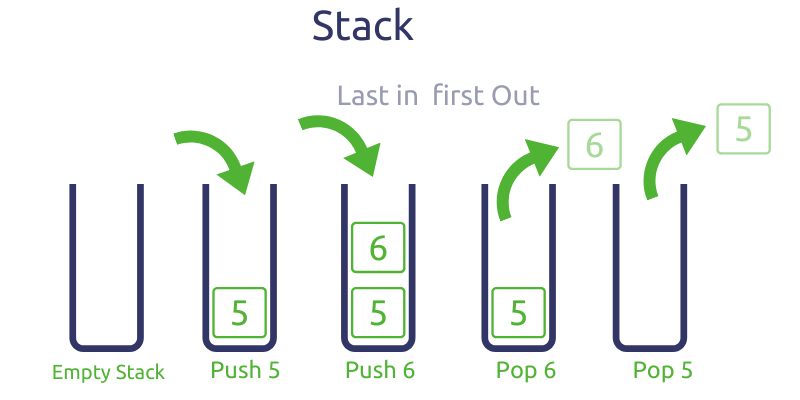
\includegraphics[width=0.7\textwidth]{figs/stack/Stack-data-structure.png}
  \end{center}

  \begin{easylist}
    & 操作系统中的栈

    && 由编译器自动分配释放 ,存放函数的参数值,局部变量的值等。栈使用的是一级缓
    存,被调用时处于存储空间中,调用完毕立即释放。

    & 数据结构中的栈

    && 一种后进先出的数据结构
  \end{easylist}
\end{frame}

\begin{frame}[fragile]
  \frametitle{为什么设计栈、研究栈?}
  \scriptsize
  \begin{itemize}
  \item 栈的一个重要应用是在程序设计中实现递归,从而使许多实际问题大大简化。
  \end{itemize}

  \begin{columns}
    \begin{column}[T]{0.5\linewidth}
      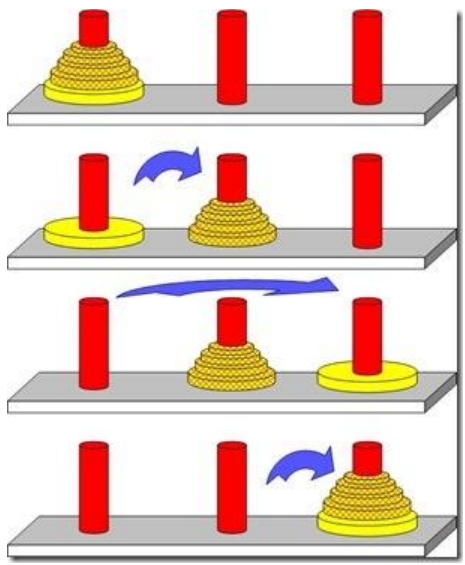
\includegraphics[width=0.9\textwidth]{figs/stack/Tower-Of-Hanoi-1.png}
    \end{column}
    \begin{column}[T]{0.5\linewidth}
        \begin{itemize}
        \item 上帝创造世界的时候做了三根金刚石柱子,在一根柱子上从下往上按大小顺
          序摞着64片黄金圆盘。上帝命令婆罗门把圆盘从下面开始按大小顺序重新摆放在
          另一根柱子上,并且规定一次只能移动一个圆盘,在小圆盘上不能放大圆盘。
        \item 有预言说,这件事完成时宇宙会在一瞬间闪电式毁灭。也有人相信婆罗门至
          今还在一刻不停地搬动着圆盘。
        \item \color{red} 18,446,744,073,709,551,615次搬动才能挪完64片金盘!
        \end{itemize}
    \end{column}
  \end{columns}
\end{frame}

\begin{frame}[fragile]
  \frametitle{举例:计算n的阶乘}
  \scriptsize
  \begin{columns}
    \begin{column}[T]{0.4\linewidth}
      \begin{minted}{java}
        int factorial (int n) {
          int  f ;
          if (n==1) f=1;
          else f=n*fact (n-1) ;
          return f;
        }
      \end{minted}
    \end{column}
    \begin{column}[T]{0.6\linewidth}
      \begin{enumerate}
      \item 将调用函数的现场(各寄存器的值,中断时的程序地址等)入栈,转入被调函数;
      \item 执行被调函数,如又调用其它函数,则执行上述步骤;
      \item 被调函数执行完,取栈顶的值,恢复调用函数时的现场,根据现场中的指令地
        址,恢复调用函数在中断处继续执行。
      \end{enumerate}
    \end{column}
  \end{columns}
  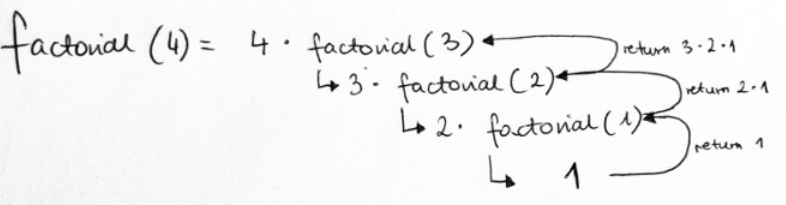
\includegraphics[width=0.9\textwidth]{figs/stack/factorial.png}
\end{frame}

\subsection{栈的存储表示方法}
\begin{frame}[fragile]
  \frametitle{栈的存储表示方法}
  \begin{tcolorbox}[colframe=red]
    请考虑其常用操作。试想选用顺序存储还是链式存储?
  \end{tcolorbox}

  \begin{columns}
    \begin{column}[T]{0.1\textwidth}
      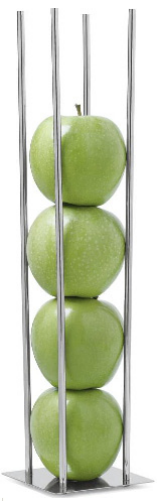
\includegraphics[width=1cm]{figs/stack/apple.png}
    \end{column}
    \begin{column}[T]{0.5\textwidth}
      \begin{easylist}
        & 特点:后进先出

        && 1、经常性的在栈顶插入新元素,以及取栈顶元素;

        && 2、无须访问非栈顶元素。
      \end{easylist}
    \end{column}
    \begin{column}[T]{0.4\textwidth}
      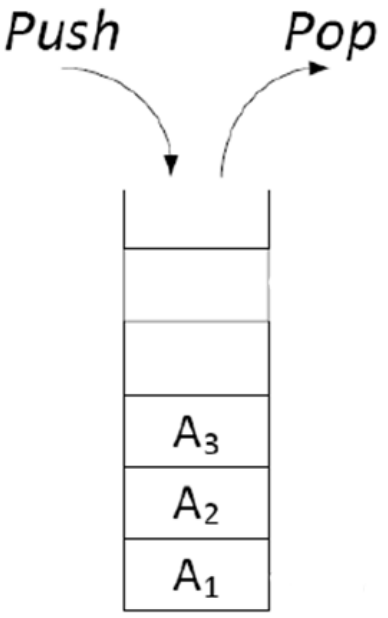
\includegraphics[width=3cm]{figs/stack/pushpop.png}
    \end{column}
  \end{columns}
\end{frame}

\begin{frame}[fragile]
  \frametitle{1. 顺序栈}
  \begin{columns}
    \begin{column}[T]{0.5\linewidth}
      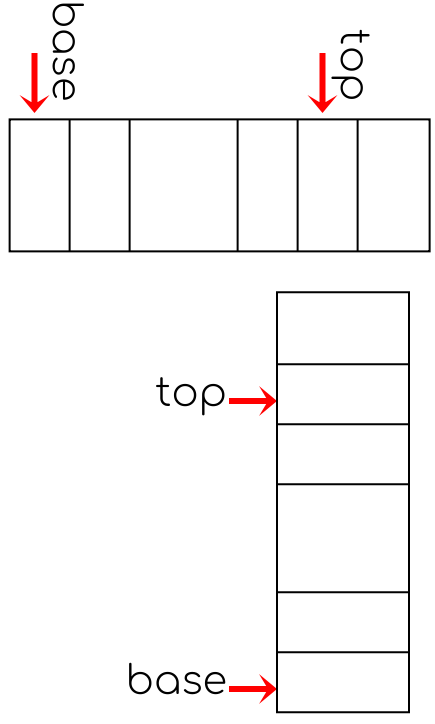
\includegraphics[width=0.7\textwidth]{figs/stack/seq-stack.png}
    \end{column}
    \begin{column}[T]{0.5\linewidth}
      \begin{enumerate}
      \item 顺序栈中元素用地址连续的存储单元依次存放;
      \item 栈底位置固定不变;
      \item 栈顶位置top随着进栈和出栈的操作而变化。
      \end{enumerate}

      顺序栈类型定义:

      \begin{minted}{c}
        class stack<Elem>{
          Object[] data;
          int top;
          int maxSize;
        } SeqStack;
      \end{minted}
    \end{column}
  \end{columns}
\end{frame}

\begin{frame}[fragile]
  \begin{easylist}
    & 动态分配
    && 先为栈分配一个初始容量,在栈的空间不够使用时再逐段扩大。

    & 指针base
    && 始终指向栈底位置,如果base为NULL表示栈不存在;

    & 指针top
    && 初值指向栈底,即top = =base,表示栈空;(不唯一)
    && 每当插入新的栈顶元素,指针top++;
    && 每当删除栈顶元素,指针top--;
    && 非空栈中的栈顶指针始终在栈顶元素的下一个位置上。
  \end{easylist}

  \centering
  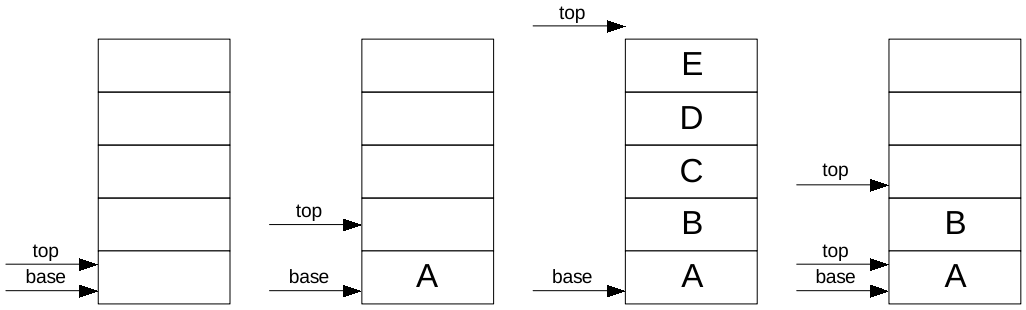
\includegraphics[width=0.8\textwidth]{figs/stack/stack-demo.png}
\end{frame}

\begin{frame}[fragile]
  \begin{columns}
    \begin{column}[T]{0.5\linewidth}
      \begin{tcolorbox}[height=8cm]
        对于顺序栈,入栈需要判栈是否满,是则需要中止、或重新分配空间,否则出现空间溢出。

        \begin{minted}{java}
public Boolean push (Elem e) {
  if ( top==maxSize) {
    print("栈已满");
    return false;
  }
  data[top++] = e;
  return true;
}
        \end{minted}
      \end{tcolorbox}
    \end{column}
    \begin{column}[T]{0.5\linewidth}
      \pause
      \begin{tcolorbox}[height=8cm]
        出栈首先要判断栈是否为空;否则栈空时进行操作将出现下溢错误。

        \begin{minted}{java}
public Elem pop() {
  if(top==base) {
    return null;
  } else {
    top = top-1
    return data[top];
  }
}
        \end{minted}
      \end{tcolorbox}
    \end{column}
  \end{columns}
\end{frame}


\subsection{链栈}
\begin{frame}[fragile]
  \frametitle{2. 链栈}

  \small

  \begin{columns}
    \begin{column}[T]{0.7\linewidth}
      \begin{easylist}
        & 链栈有无栈满溢出问题?

        & 指针如何指?

        && 从栈顶依次向后指,因为操作主要是在栈顶插入、删除,经常需要根据栈顶元
        素找次顶元素。

        & 是否要加头结点?

        && No. 因为头部插入不会出现处理不一致的问题.
      \end{easylist}

      写出链栈的类型定义:

      \begin{minted}{java}
        class Node{
          Elem data;
          Node next;
        }

        Node  top ; // 链栈
      \end{minted}
    \end{column}
    \begin{column}[T]{0.3\linewidth}
      \scalebox{0.8}{
        \begin{tikzpicture}[fill=red, box/.style={draw, minimum width=0.85cm, minimum height=0.8cm, fill=red!5}]
	        \draw node[] (base) {$base$}
          node[box, thick, right=of base] (d1) { 9 }   node[box, right=0 of d1] (p1) {}
          node[box, above=of d1] (d2) {45}  node[box, right=0 of d2] (p2) {}
          node[box, above=of d2] (d3) {25}  node[box, right=0 of d3] (p3) {$\wedge$}
	        node[left= of d3] (top) {$top$};

          \path (base) edge[draw, dashed, thick, ->] (d1) (top) edge[draw=red, thick, ->] (d3);
		      \path (p1.center) edge[draw=red,  thick, ->, out=45, in=200] (d2) (p2.center) edge[draw=red, thick, in=200, ->] (d3);
        \end{tikzpicture}
      }
    \end{column}
  \end{columns}
\end{frame}

\begin{frame}[fragile]
% \frametitle{链栈基本操作}

  请尝试写出入栈出栈的算法

  \begin{minted}{java}
    public push (Elem e) {
      //是否还要判断栈是否满?
      top=new Node(e, top);
      return OK;
   }

   public pop( ){
     //是否还要判断栈是否空?
     e=top;
     top=top.next;
     e.next=null;
     return e.data;
}
  \end{minted}

\end{frame}

\begin{frame}[fragile]
  \frametitle{栈的应用}
  迷宫求解(见PPT)
\end{frame}

\section{队列}

\begin{frame}[fragile]
  \frametitle{队/Queue}
   \begin{columns}
    \begin{column}[T]{0.5\linewidth}
      \begin{tcolorbox}[colframe=blue!80, height=6.5cm, title=队/Queue]
        \small
        \begin{itemize}
        \item 限制仅在表的一端进行插入、在另一端进行删除。
        \item 允许插入的一端称队尾 (rear),允许删除的一段称为队头 (front)。
        \item FIFO:First In First Out
        \end{itemize}
      \end{tcolorbox}
    \end{column}
    \begin{column}[T]{0.5\linewidth}
      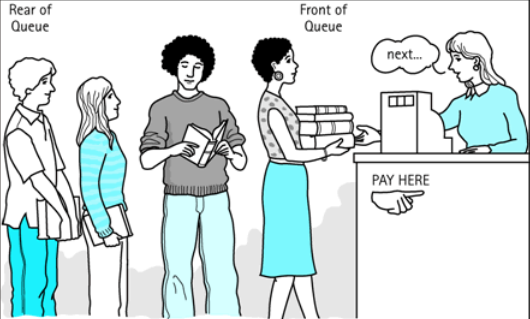
\includegraphics[width=0.9\textwidth]{figs/queue/queueofpeople.png}

      \begin{itemize}
      \item 比如生活中排队购物、操作系统中的作业排队等。
      \end{itemize}
    \end{column}
  \end{columns}
\end{frame}


\subsection{队的存储表示方法}
\begin{frame}[fragile]
  \frametitle{队的存储表示方法}

  \begin{itemize}
  \item 队也有两种存储表示方法:顺序队、链队
  \item 顺序队:利用地址连续的存储单元依次存放数据元素。
  \end{itemize}

  \begin{columns}
    \begin{column}[T]{0.5\linewidth}
      \scalebox{0.6}{
        \begin{tikzpicture}[scale=0.5, box/.style={draw, minimum width=1.2cm, minimum height=0.7cm}]
		      \draw node[box] (a0) {A}
	        node[box, right=0 of a0] (a1) {B}
	        node[box, right=0 of a1] (a2) {C}
	        node[box, right=0 of a2] (a3) {}
          node[box, right=0 of a3, minimum width=2cm] (amore) {$\cdots$}
	        node[box, right=0 of amore] (alast) {}
		      node[above=0 of a0] {0}
				  node[above=0 of a1] {1}
				  node[above=0 of a2] {2}
				  node[above=0 of a3] {3}
				  node[above=0 of amore] {$\cdots$}
				  node[above=0 of alast] {$MaxLen-1$}
	        node[below=0.7cm of a0] (front) {$front$}
	        node[below=0.7cm of a2] (rear) {$rear$};

			    \draw[draw=red, thick, -Latex] (front) -> (a0);
          \draw[draw=red, thick, -Latex] (rear) -> (a2);
        \end{tikzpicture}
      }
    \end{column}
    \begin{column}[T]{0.5\linewidth}
      请写出顺序队的类型定义:

      \begin{minted}{java}
        class SeqQueue{
          ElemType  data[ ];
          int maxsize;
          int rear; //队尾,以此计算队长
        }
      \end{minted}

       可否??
    \end{column}
  \end{columns}
\end{frame}

\begin{frame}[fragile]
  \frametitle{顺序队的基本操作}
  \begin{easylist}
    & 入队:如有空间,元素$x$入队后队尾指针加1

    && data[rear++]=x;

    & 出队:如有元素,队头指针加1,表明队头元素出队。

    && x=sq.data[sq.front++];
  \end{easylist}

  \vspace{1cm}

  \begin{tikzpicture}[scale=0.5, box/.style={draw, minimum width=1.2cm, minimum height=0.7cm}]
		\draw node[box] (a0) {A}
	  node[box, right=0 of a0] (a1) {B}
	  node[box, right=0 of a1] (a2) {C}
	  node[box, right=0 of a2] (a3) {}
    node[box, right=0 of a3, minimum width=2cm] (amore) {$\cdots$}
	  node[box, right=0 of amore] (alast) {}
		node[above=0 of a0] {0}
		node[above=0 of a1] {1}
		node[above=0 of a2] {2}
		node[above=0 of a3] {3}
		node[above=0 of amore] {$\cdots$}
		node[above=0 of alast] {$MaxLen-1$}
	  node[below=0.7cm of a0] (front) {$front$}
	  node[below=0.7cm of a2] (rear) {$rear$};

		\draw[draw=red, thick, -Latex] (front) -> (a0);
    \draw[draw=red, thick, -Latex] (rear) -> (a2);
  \end{tikzpicture}
\end{frame}

\begin{frame}[fragile]
  \scriptsize
  \begin{itemize}
  \item 设maxsize=10。请你写出如下状态或执行某操作后的顺序队元素。
    \begin{enumerate}
    \item 空队;
    \item a0, a1, a2依次入队;
    \item a3, a4, a5, a6, a7, a8依次入队, a0, a1, a2, a3, a4, a5依次出队;
    \item a9, a10入队。
    \end{enumerate}
  \end{itemize}

  \begin{columns}
    \begin{column}[T]{0.2\linewidth}
      \scalebox{0.8}{
        \begin{tikzpicture}[scale=0.5, box/.style={draw, minimum width=1cm, minimum height=0.5cm}]
          \draw node[box] (a0) {} node[left=0.2cm of a0]{0};
          \foreach \i in {1,...,9} {
            \pgfmathtruncatemacro{\x}{\i - 1};
            \draw node[box, above=0 of a\x] (a\i) {} node[left=0.2cm of a\i]{\i};
          }

          \draw node[left=1cm of a0, yshift=0.5cm] (front) {front}  node[left=1cm of a0, yshift=-0.5cm] (rear) {rear};
          \draw[draw=red, thick, -Latex] (front) -> (a0);
          \draw[draw=red, thick, -Latex] (rear) -> (a0);
        \end{tikzpicture}
      }

      (a) 空队
    \end{column}
    \begin{column}[T]{0.2\linewidth}
      \scalebox{0.8}{
        \begin{tikzpicture}[scale=0.5, box/.style={draw, minimum width=1cm, minimum height=0.5cm}]
          \draw node[box] (a0) {$a_0$} node[left=0.2cm of a0]{0};
          \foreach \i in {1,...,2} {
            \pgfmathtruncatemacro{\x}{\i - 1};
            \draw node[box, above=0 of a\x] (a\i) {$a_\i$} node[left=0.2cm of a\i]{\i};
          }
          \foreach \i in {3,...,9} {
            \pgfmathtruncatemacro{\x}{\i - 1};
            \draw node[box, above=0 of a\x] (a\i) {} node[left=0.2cm of a\i]{\i};
          }

          \draw node[left=1.5cm of a0] (front) {}  node[left=1.5cm of a3] (rear) {};
          \path[] (front)  edge[draw=red, thick, -Latex, above left] node{front} (a0);
          \path[] (rear)  edge[draw=red, thick, -Latex, above left] node{rear} (a3);
        \end{tikzpicture}
      }

      (b) 有3个元素
    \end{column}
    \begin{column}[T]{0.2\linewidth}
      \scalebox{0.8}{
        \begin{tikzpicture}[scale=0.5, box/.style={draw, minimum width=1cm, minimum height=0.5cm}]
          \draw node[box] (a0) {} node[left=0.2cm of a0]{0};
          \foreach \i in {1,...,5} {
            \pgfmathtruncatemacro{\x}{\i - 1};
            \draw node[box, above=0 of a\x] (a\i) {} node[left=0.2cm of a\i]{\i};
          }
          \foreach \i in {6,...,8} {
            \pgfmathtruncatemacro{\x}{\i - 1};
            \draw node[box, above=0 of a\x] (a\i) {$a_\i$} node[left=0.2cm of a\i]{\i};
          }
          \foreach \i in {9,...,9} {
            \pgfmathtruncatemacro{\x}{\i - 1};
            \draw node[box, above=0 of a\x] (a\i) {} node[left=0.2cm of a\i]{\i};
          }

          \draw node[left=1.5cm of a6] (front) {}  node[left=1.5cm of a9] (rear) {};
          \path[] (front)  edge[draw=red, thick, -Latex, above left] node{front} (a6);
          \path[] (rear)  edge[draw=red, thick, -Latex, above left] node{rear} (a9);
        \end{tikzpicture}
      }

      (c) 一般情况
    \end{column}
    \begin{column}[T]{0.2\linewidth}
      \scalebox{0.8}{
        \begin{tikzpicture}[scale=0.5, box/.style={draw, minimum width=1cm, minimum height=0.5cm}]
          \draw node[box] (a0) {} node[left=0.2cm of a0]{0};
          \foreach \i in {1,...,5} {
            \pgfmathtruncatemacro{\x}{\i - 1};
            \draw node[box, above=0 of a\x] (a\i) {} node[left=0.2cm of a\i]{\i};
          }
          \foreach \i in {6,...,9} {
            \pgfmathtruncatemacro{\x}{\i - 1};
            \draw node[box, above=0 of a\x] (a\i) {$a_\i$} node[left=0.2cm of a\i]{\i};
          }

          \draw node[left=1.5cm of a6] (front) {}  node[left=1.5cm of a9, yshift=0.5cm] (rear) {};
          \path[] (front)  edge[draw=red, thick, -Latex, above left] node{front} (a6);
          \path[] (rear)  edge[draw=red, thick, -Latex, above left] node{rear} ++(3,0);
        \end{tikzpicture}
      }

      (d) 假溢出现象
    \end{column}
    \begin{column}[T]{0.2\linewidth}
      \pause
      \begin{itemize}
      \item 入队出队会使整个队列整体后移
      \item “假溢出”: 队尾指针已经移到了最后,不能再执行入队操作,但此时队中并未
        真的“满员” 。如何解决这个问题?
      \end{itemize}
    \end{column}
  \end{columns}
\end{frame}

\begin{frame}[fragile]
  \frametitle{}
  \begin{itemize}
  \item Linear Queue入队出队会使整个队列整体后移
  \item “假溢出”: 队尾指针已经移到了最后,不能再执行入队操作,但此时队中并未
    真的“满员” 。如何解决这个问题?
    \begin{enumerate}
    \item 平移元素;
    \item {\color{red}循环队列 (Circular Queue):将顺序队列的存储区假想为环状空
      间。}在假溢出时,将新元素插入到第一个位置上,这样做,虽物理上队尾在队首之
      前,但逻辑上队首仍然在前。入列和出列仍按“先进先出”的原则进行。

      \begin{itemize}
      \item 入队时的队尾指针操作: \\
        rear=(rear+1) \% maxsize;
      \item 出队时的队头指针操作:\\
		    front=(front+1) \% maxsize;
      \end{itemize}
    \end{enumerate}
  \end{itemize}
\end{frame}

\begin{frame}[fragile]
  \frametitle{循环队列 (Circular Queue)\footnote{延伸阅读:\url{https://en.wikipedia.org/wiki/Circular\_buffer}
  }}
  \small
  \begin{itemize}
  \item head/front points to the first (oldest) used element --- the next element to be read
  \item tail/rear points to the first (oldest) unused element --- the next element to be written
  \item rear: 多数情况下指向尾部元素,tail: 多数情况下指向尾部的下一个元素。教材
    中的rear等同于tail
  \end{itemize}

  \begin{columns}
    \begin{column}[T]{0.5\linewidth}
      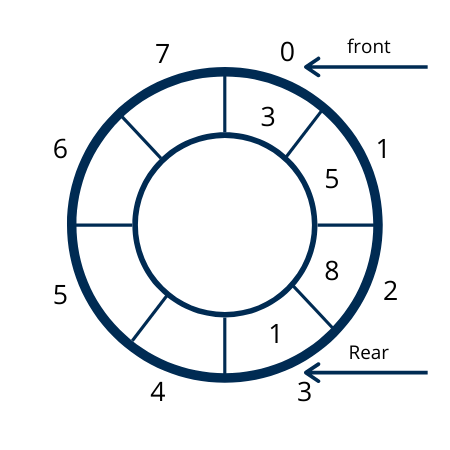
\includegraphics[width=0.55\textwidth]{figs/stack/circular-queue-1.png}
    \end{column}
    \begin{column}[T]{0.5\linewidth}
      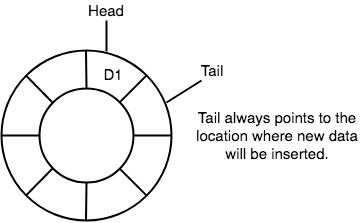
\includegraphics[width=0.75\textwidth]{figs/stack/circular-queue-2.png}
    \end{column}
  \end{columns}
\end{frame}

\begin{frame}[fragile]
  \begin{easylist}
    & 设maxsize=10。队列状态如(a)所示。请写出分别执行如下操作后的front和rear值:
    && 情况1: a9, a10, a11, a12, a13, a14依次入队
    && 情况2: a5, a6, a7, a8依次出队
  \end{easylist}

  \pause

  \centering
  \begin{columns}
    \begin{column}[T]{0.3\linewidth}
      (a) 有4个元素

      \scalebox{0.8}{
        \begin{tikzpicture}[scale=0.5, box/.style={draw, minimum width=1cm, minimum height=0.5cm}]
          \draw node[box] (a0) {} node[left=0.2cm of a0]{0};
          \foreach \i in {1,...,4} {
            \pgfmathtruncatemacro{\x}{\i - 1};
            \draw node[box, above=0 of a\x] (a\i) {} node[left=0.2cm of a\i]{\i};
          }
          \foreach \i in {5,...,8} {
            \pgfmathtruncatemacro{\x}{\i - 1};
            \draw node[box, above=0 of a\x] (a\i) {$a_\i$} node[left=0.2cm of a\i]{\i};
          }
          \foreach \i in {9,...,9} {
            \pgfmathtruncatemacro{\x}{\i - 1};
            \draw node[box, above=0 of a\x] (a\i) {} node[left=0.2cm of a\i]{\i};
          }
          \draw node[left=1.5cm of a5] (front) {}  node[left=1.5cm of a8, yshift=0.5cm] (rear) {};
          \path[] (front)  edge[draw=red, thick, -Latex, above left] node{front} (a5);
          \path[] (rear)  edge[draw=red, thick, -Latex, above left] node{rear}  (a9);
        \end{tikzpicture}
      }
    \end{column}
    \begin{column}[T]{0.4\linewidth}
      (b) 情况1:队满

      \scalebox{0.8}{
        \begin{tikzpicture}[scale=0.5, box/.style={draw, minimum width=1cm, minimum height=0.5cm}]
          \draw node[box] (a0) {$a_{10}$} node[left=0.2cm of a0]{0};
          \foreach \i in {1,...,4} {
            \pgfmathtruncatemacro{\x}{\i - 1};
            \pgfmathtruncatemacro{\v}{\i + 10};
            \draw node[box, above=0 of a\x] (a\i) {$a_{\v}$} node[left=0.2cm of a\i]{\i};
          }
          \foreach \i in {5,...,9} {
            \pgfmathtruncatemacro{\x}{\i - 1};
            \draw node[box, above=0 of a\x] (a\i) {$a_\i$} node[left=0.2cm of a\i]{\i};
          }

          \draw node[left=1cm of a5,yshift=0.25cm] (front) {front}  node[left=1cm of a5,  yshift=-0.25cm] (rear) {rear};
          \path[] (front.east)  edge[draw=red, thick, -Latex,  in=155] node{}  (a5.west);
          \path[] (rear.east)  edge[draw=red, thick, -Latex, in=205] node{}   (a5.west);
        \end{tikzpicture}
      }

    \end{column}
    \begin{column}[T]{0.3\linewidth}
      (c) 情况2:队空

      \scalebox{0.8}{
        \begin{tikzpicture}[scale=0.5, box/.style={draw, minimum width=1cm, minimum height=0.5cm}]
          \draw node[box] (a0) {} node[left=0.2cm of a0]{0};
          \foreach \i in {1,...,9} {
            \pgfmathtruncatemacro{\x}{\i - 1};
            \draw node[box, above=0 of a\x] (a\i) {} node[left=0.2cm of a\i]{\i};
          }

          \draw node[left=1cm of a9,yshift=0.25cm] (front) {front}  node[left=1cm of a9,  yshift=-0.25cm] (rear) {rear};
          \path[] (front.east)  edge[draw=red, thick, -Latex,  in=155] node{}  (a9.west);
          \path[] (rear.east)  edge[draw=red, thick, -Latex, in=205] node{}   (a9.west);
        \end{tikzpicture}
      }
    \end{column}
  \end{columns}

  当front=rear, 队满还是队空?如何判断队满?如何判断队空?
\end{frame}

\begin{frame}[fragile]
  \frametitle{循环队的队满判别}

  \begin{columns}
    \begin{column}[T]{0.7\linewidth}
      \begin{easylist}
        & 方法一

        && 附设一个存储队中元素个数的变量如num,当num=0时队空,当num=maxsize时为
        队满。

        & 方法二

        && 少用一个元素空间,把右图所示情况视为队满,此时的状态是队尾指针加1就会
        从后面赶上队头指针: (rear+1) \% maxsize==front,从而和空队区别开来。
      \end{easylist}
    \end{column}
    \begin{column}[T]{0.3\linewidth}
      \begin{tikzpicture}[scale=0.5, box/.style={draw, minimum width=1cm, minimum height=0.5cm}]
        \draw node[box] (a0) {$a_{10}$} node[left=0.2cm of a0]{0};
        \foreach \i in {1,...,3} {
          \pgfmathtruncatemacro{\x}{\i - 1};
          \pgfmathtruncatemacro{\v}{\i + 10};
          \draw node[box, above=0 of a\x] (a\i) {$a_{\v}$} node[left=0.2cm of a\i]{\i};
        }
        \draw node[box, above=0 of a3] (a4) {} node[left=0.2cm of a4]{4};
        \foreach \i in {5,...,9} {
          \pgfmathtruncatemacro{\x}{\i - 1};
          \draw node[box, above=0 of a\x] (a\i) {$a_\i$} node[left=0.2cm of a\i]{\i};
        }

        \draw node[left=1cm of a5] (front) {front}  node[left=1cm of a4] (rear) {rear};
        \path[] (front)  edge[draw=red, thick, -Latex, left] node{}  ++ (3,0);
        \path[] (rear)  edge[draw=blue, thick, -Latex, left] node{}   ++ (3,0);
      \end{tikzpicture}
    \end{column}
  \end{columns}
\end{frame}

\begin{frame}[fragile]
  \frametitle{循环队的基本操作}
  \scriptsize
  \begin{minted}{java}
    class SeqQueue  {
      ElemType data[];
      int maxsize;
      int front, rear;  /*队头队尾指针*/
      int num;          /*队中元素的个数*/
    }

    // 入队
    int InQueue (ElemType  x){
      if  (num==maxsize) {
        printf("队满");  return 0;
      } else {
        data[rear]=x;
        rear=(rear+1) % maxsize;
        num++;
        return 1;    /*入队完成*/
      }
    }
  \end{minted}
\end{frame}

\begin{frame}[fragile]
  \frametitle{循环队的基本操作}
  \scriptsize
  \begin{minted}{java}
    //出队
    int OutQueue (ElemType  x) {
      if  (num==0) {
        printf("队空");
        return –1;
      } else {
        x=data[front];  /*读出队头元素*/
        front=(front+1) % maxsize;
        num--;
        return 1;    /*出队完成*/
      }
    }
  \end{minted}
\end{frame}


\begin{frame}[fragile]
  Python:

  \scriptsize
  \begin{minted}{python}
class SeqQueue:
    def __init__(self, max_size=10):
        self.max_size = max_size + 1 # 实际多放一个空间,区分对空、队满
        self.front = 0
        self.rear = 0
        self.elements = [None]*max_size

    def enqueue(self, element) -> bool:
        if (self.rear + 1) % self.max_size == self.front:
            print('Queue is Full!')
            return False
        else:
            self.elements[self.rear] = element
            self.rear = (self.rear + 1) % self.max_size
            return True

    def dequeue(self):
        if self.front == self.rear:
            print('Queue is Empty!')
            return None
        else:
            e = self.elements[self.front]
            self.front = (self.front + 1) % self.max_size
            return e
  \end{minted}
\end{frame}


\begin{frame}[fragile]
  \frametitle{链队}
  \begin{center}
  \begin{tikzpicture}[scale=0.5, box/.style={draw, minimum width=0.6cm, minimum height=0.5cm}]
    \draw node[box] (data0) {} node[box, right=0 of data0](link0){};
    \draw node[box, right=0.5 of link0] (data1) {$a_1$} node[box, right=0 of data1](link1){};
    \draw node[box, right=0.5 of link1] (data2) {$a_2$} node[box, right=0 of data2](link2){};
    \draw node[right=0.5 of link2] (more) {$\cdots$} ;
    \draw node[box, right=0.5 of more] (datan) {$a_n$} node[box, right=0 of datan](linkn){};
    \draw node[left=0.5cm of data0] (front) {front} node[below=0.5 of datan] (rear) {rear};

    \path[] (link0.center)  edge[draw, -Latex] node{}  (data1)
    (link1.center)  edge[draw, -Latex] node{}  (data2)
    (link2.center)  edge[draw, -Latex] node{}  (more)
    (more)  edge[draw, -Latex] node{}  (datan)
    (front) edge[draw=black!40, -Latex] (data0)
    (rear) edge[draw=black!40, -Latex] (datan);
  \end{tikzpicture}
\end{center}


  \begin{easylist}
    & 带头结点吗?
    & 尾指针rear指向队尾元素,提高插入操作效率
    & 请写出链队的类型定义
  \end{easylist}

  \begin{minted}{java}
    class QNode{
      ElemType  data;
      QNode next;
    }
    class LQueue{
      Node head, rear;
    }
  \end{minted}
\end{frame}

\begin{frame}[fragile]
  \frametitle{链队的基本操作 --- 入队}
  \begin{center}
  \begin{tikzpicture}[scale=0.5, box/.style={draw, minimum width=0.6cm, minimum height=0.5cm}]
    \draw node[box] (data0) {} node[box, right=0 of data0](link0){};
    \draw node[box, right=0.5 of link0] (data1) {$a_1$} node[box, right=0 of data1](link1){};
    \draw node[box, right=0.5 of link1] (data2) {$a_2$} node[box, right=0 of data2](link2){};
    \draw node[right=0.5 of link2] (more) {$\cdots$} ;
    \draw node[box, right=0.5 of more] (datan) {$a_n$} node[box, right=0 of datan](linkn){};
    \draw node[left=0.5cm of data0] (front) {front} node[below=0.5 of datan] (rear) {rear};

    \path[] (link0.center)  edge[draw, -Latex] node{}  (data1)
    (link1.center)  edge[draw, -Latex] node{}  (data2)
    (link2.center)  edge[draw, -Latex] node{}  (more)
    (more)  edge[draw, -Latex] node{}  (datan)
    (front) edge[draw=black!40, -Latex] (data0)
    (rear) edge[draw=black!40, -Latex] (datan);
  \end{tikzpicture}
\end{center}


  \begin{minted}{java}
    void InQueue(ElemType  x) {
      rear.next=new QNode(x,null);
      rear=rear.next;
    }
  \end{minted}
\end{frame}

\begin{frame}[fragile]
  \frametitle{链队的基本操作 --- 出队}
  \begin{center}
  \begin{tikzpicture}[scale=0.5, box/.style={draw, minimum width=0.6cm, minimum height=0.5cm}]
    \draw node[box] (data0) {} node[box, right=0 of data0](link0){};
    \draw node[box, right=0.5 of link0] (data1) {$a_1$} node[box, right=0 of data1](link1){};
    \draw node[box, right=0.5 of link1] (data2) {$a_2$} node[box, right=0 of data2](link2){};
    \draw node[right=0.5 of link2] (more) {$\cdots$} ;
    \draw node[box, right=0.5 of more] (datan) {$a_n$} node[box, right=0 of datan](linkn){};
    \draw node[left=0.5cm of data0] (front) {front} node[below=0.5 of datan] (rear) {rear};

    \path[] (link0.center)  edge[draw, -Latex] node{}  (data1)
    (link1.center)  edge[draw, -Latex] node{}  (data2)
    (link2.center)  edge[draw, -Latex] node{}  (more)
    (more)  edge[draw, -Latex] node{}  (datan)
    (front) edge[draw=black!40, -Latex] (data0)
    (rear) edge[draw=black!40, -Latex] (datan);
  \end{tikzpicture}
\end{center}


  \begin{minted}{java}
    ElemType OutQueue() {
      QNode p;
      if (front==rear) {
        printf ("队空");
        return null;
      } else {
        p=front.next;    //把队的第一个结点取出
        front.next=p.next;   //把队头直接指向原第二个结点
        e=p.data;       /*队头元素放e中*/
        if (front.next==NULL)
          rear=front;  //若只有一个元素,出队后队空,需修改队尾指针
        return e;
      }
    }
  \end{minted}
\end{frame}


\subsection{队列应用}

\begin{frame}[fragile]
  \frametitle{队列应用 --- 迷宫寻路}
  \begin{columns}
    \begin{column}[T]{0.6\linewidth}
      \begin{easylist}
        & 从迷宫入口点(1,1)出发,向四周搜索,记下所有一步能到达的坐标点;然后
        依次再从这些点出发,再记下所有一步能到达的坐标点,…,依此类推,直到到达
        迷宫的出口点(8,8)为止,然后从出口点沿搜索路径回溯直至入口。这样就找到了
        一条迷宫的最短路径,否则迷宫无路径。

        & 与基于栈的迷宫求解的异同?
      \end{easylist}
    \end{column}
    \begin{column}[T]{0.4\linewidth}
      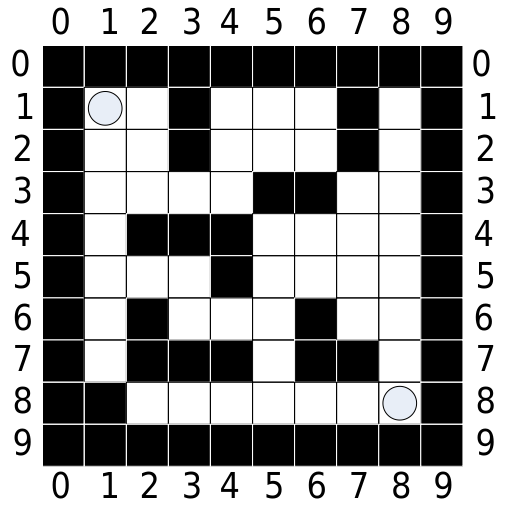
\includegraphics[width=0.8\textwidth]{figs/stack/maze.png}
    \end{column}
  \end{columns}
\end{frame}

\begin{frame}[fragile]
  \frametitle{解法图示}
  \begin{columns}
    \begin{column}[T]{0.6\linewidth}
      \scalebox{0.8}{
        \begin{forest}
          for tree={draw, rectangle, rounded corners},
          [ {(1, 1)},
            [{(1,2)} [{(2,2)} [{(3,2)}]] ]
            [{(2,1)} [{(2,2)}, fill=yellow!50]  [{(3,1)} [{(3,2), fill=yellow!50}] [{(4,1)}]]]
          ]
        \end{forest}
      }
      \begin{easylist}
        & 上述处理的实质:
        && 对可通行路径的空间的\color{red}广度优先搜索
        & 如何向前摸索?
        & 到达出口后,如何回溯?
      \end{easylist}
    \end{column}
    \begin{column}[T]{0.4\linewidth}
      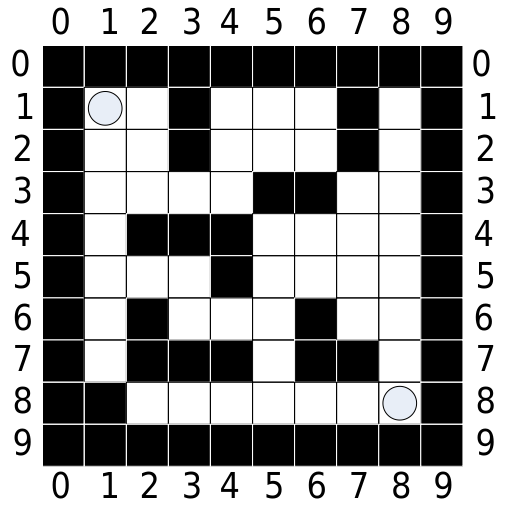
\includegraphics[width=0.8\textwidth]{figs/stack/maze.png}
    \end{column}
  \end{columns}
\end{frame}

\begin{frame}[fragile]
  \frametitle{解法图示}
  \begin{columns}
    \begin{column}[T]{0.6\linewidth}
      \begin{easylist}
        & 如何向出口摸索:搜索路径的存储1

        && 在搜索过程中必须记下每一个可到达的坐标点,以便从这些点出发继续向四周搜索,
        使用 “FIFO”的队列保存已到达的点即可.

        & 如何向入口回溯:搜索路径的存储2

        && 为了能够从出口点沿搜索路径回溯直至入口,对于每一点,记下坐标点的同时,还
        要记下到达该点的前驱点或者从前驱点来的方向(8个方向之一)。
      \end{easylist}
    \end{column}
    \begin{column}[T]{0.4\linewidth}
      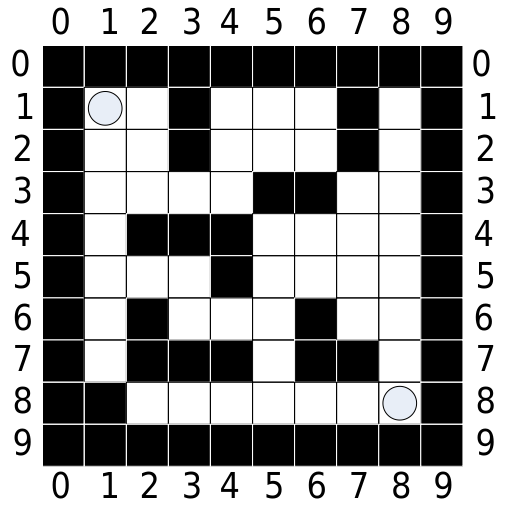
\includegraphics[width=0.8\textwidth]{figs/stack/maze.png}
    \end{column}
  \end{columns}
\end{frame}
